\documentclass[12pt,a4paper]{article}

% --- Packages ---
\usepackage[utf8]{inputenc}          % UTF-8 encoding
\usepackage[T1]{fontenc}             % Font encoding
\usepackage{lmodern}                 % Better fonts
\usepackage{amsmath, amssymb, amsfonts} % Math symbols
\usepackage{mathtools}               % Extra math tools
\usepackage{geometry}                % Page layout
\geometry{margin=1in}

\usepackage{hyperref}                % Links in PDF
\usepackage{graphicx}                % Images
\usepackage{float}                   % Force figure placement
\usepackage{caption}                 % Captions for figures/tables
\usepackage{subcaption}              % Subfigures
\usepackage{tikz}                    % Diagrams
\usetikzlibrary{arrows,positioning}

\usepackage{algorithm}               % Algorithms
\usepackage{algpseudocode}           % Pseudocode
\usepackage{listings}                % Code listings
\usepackage{xcolor}                  % Colors for code

\setlength{\headheight}{15pt}

\usepackage[listings]{tcolorbox}
\tcbuselibrary{listings,theorems}

% Definition theorem-style box
\newtcbtheorem[number within=section]{definition}{Definition}%
{colback=blue!5,colframe=blue!35!black,fonttitle=\bfseries}{def}

\newcommand{\newpar} {
  \vspace{1em}
  \noindent
}

\newcommand{\bemph}[1]{\textbf{\emph{#1}}}

\newcommand{\dq}[1]{``#1''}
\newcommand{\sq}[1]{`#1'}

\lstset{
    basicstyle=\ttfamily,      % monospaced font
    columns=fullflexible,      % fixes spacing issues
    keepspaces=true,           % preserve spaces
    showstringspaces=false
    language=Python,
    keywordstyle=\color{blue}\bfseries,
    commentstyle=\color{green},
    stringstyle=\color{red},
}

% --- Headers ---
\usepackage{fancyhdr}
\pagestyle{fancy}
\fancyhf{}
\lhead{CS/Math Notes}
\rhead{\today}
\cfoot{\thepage}

% --- Title ---
\title{Notes on Crafting Interpreters by Robert Nystrom}
\author{Jason Mac}

\begin{document}

\maketitle
\tableofcontents
\newpage

% --- Sections ---
\section{Parts of a Language and the Lox Language}

\subsection{Overview}


\textbf{Credit:} Robert Nystrom,
\href{https://craftinginterpreters.com/}{\textit{Crafting Interpreters}}.
This set of notes is directly sourced from this book as linked.
It is an extremely well crafted text that gives a concise, yet extremely insightful introduction to
creating your own progmamming language.

A language can be broken up into many parts. This set of notes taken from Crafting Interpreters is concerned about its impementation.
In particular, we will be creating an interpreter for the Lox language as created by Robert Nystrom using C\#.
A language's impementation can be pieced down into separate parts. It's useful to make the abstraction to create intermediate representation
of the source code to remain indendent of the system we are compiling or interpreting on.
The remainder of section will give an overview on the Lox langauge and its specifications.



\subsection{Hello, Lox}

Your first Lox program:

\begin{lstlisting}
// Print "Hello, world!" in Lox
print "Hello, world!";
\end{lstlisting}

Lox has C-family syntax: semicolons end statements, 'print' is a built-in statement, and parentheses are generally not required around arguments.

\subsection{A High-Level Language}

Lox is small, high-level, and dynamically typed. Its design is inspired by languages like JavaScript, Scheme, and Lua:

\subsubsection{Dynamic Typing}
Variables can store values of any type and change type at runtime. Type errors are detected only when code executes.
The author states that, although static typing is useful in many scenarios, it is more trouble that it's worth to implement it
for the core learning purposes.

\subsubsection{Automatic Memory Management}
Memory is handled automatically via garbage collection. Lox avoids manual allocation and deallocation, simplifying programming.
The implemntation of the garbage collector will be done by us.

\subsection{Data Types}

Lox supports a small set of built-in types:

\begin{itemize}
	\item \textbf{Booleans}: \texttt{true}, \texttt{false}
	\item \textbf{Numbers}: double-precision floating point, e.g., \texttt{1234;} or \texttt{12.34;}
	\item \textbf{Strings}: enclosed in double quotes, e.g., \texttt{"Hello"}
	\item \textbf{Nil}: represents absence of a value (\texttt{nil})
\end{itemize}

It is stated that it is more trouble than its worth to ban the \texttt{nil} value from the language since it is dynamically typed. It is interesting to note that
the introduction of the \texttt{null} value in C is considered the \textbf{"billion-dollar mistake"} by Tony Hoare, its own inventor.

\subsection{Expressions}

Expressions combine literals and operators to produce values.
If built-in data types and their literals are atoms, then expressions must be the molecules.
For example, an arithmetic expression in Lox could be:

\begin{verbatim}
1 + 2 * 3
\end{verbatim}

Here, "1", "2", and "3" are literals, and "+" and "*" are operators combining them into an expression.

\subsubsection{Arithmetic}
Lox has the basic arithmetic operators that are common to many languages, perhaps necessary to be turing-complete.
\begin{lstlisting}
add + me;
subtract - me;
multiply * me;
divide / me;
-negateMe;
\end{lstlisting}
\textbf{Operands and Operators:}
\begin{itemize}
	\item \textbf{Operand:} A value that an operator acts on. Example: in \texttt{3 + 4}, both \texttt{3} and \texttt{4} are operands.
	\item \textbf{Binary operator:} An operator with two operands. Example: \texttt{+}, \texttt{-}, \texttt{*}, \texttt{/}.
	\item \textbf{Infix operator:} Operator appears \textbf{between} operands. Example: \texttt{3 + 4}.
	\item \textbf{Prefix operator:} Operator appears \textbf{before} its operand. Example: \texttt{-5}.
	\item \textbf{Postfix operator:} Operator appears \textbf{after} its operand. Example: \texttt{i++} in C.
\end{itemize}

\subsubsection{Comparison and Equality}
Lox includes comparison operators that will produce a true or false value.
\begin{lstlisting}
less < than;
lessThan <= orEqual;
greater > than;
greaterThan >= orEqual;
\end{lstlisting}
\textbf{Equality and Inequality:}
\begin{itemize}
	\item Compare any values with \texttt{==} (equals) or \texttt{!=} (not equals).
	\item Examples:
	      \begin{itemize}
		      \item \texttt{1 == 2} \(\rightarrow\) false
		      \item \texttt{"cat" != "dog"} \(\rightarrow\) true
		      \item \texttt{314 == "pi"} \(\rightarrow\) false
		      \item \texttt{123 == "123"} \(\rightarrow\) false
	      \end{itemize}
	\item Values of different types are never equivalent; no implicit conversions.
\end{itemize}


\subsubsection{Logical Operators}
Lox provides negation of booleans through the prefix operator \texttt{!} and works as expected.
The conjunction and disjunction of statements is done with binary operators, \texttt{and}, \texttt{or}.
These are control flow statements.

\noindent In particular, \texttt{and} returns its left operand if its false, otherwise it returns its right operand.

\noindent Similarly, \texttt{or} returns its left operand if its true, otherwise it returns its right operand.

\noindent The operator is a short circuit.
\begin{lstlisting}
!true;       // false
true and false; // false
true or false;  // true
\end{lstlisting}

\subsection{Statements}

\textbf{Statements:} Produce effects rather than values (unlike expressions).
Statments, as metioned by Nystrom, by definition, don't evaluate to value.
To be useful, they must either modify some state, read input, or produce output.

\noindent- \texttt{print "Hello, world!";} → evaluates expression and displays the result (produce output)

\noindent- Expression statement: an expression followed by \texttt{;} is promoted to a statement.

\noindent Example: \texttt{"some expression";}

\noindent - \textbf{Blocks:} Wrap multiple statements in \texttt{\{ … \}}. Blocks affect scoping.
\begin{lstlisting}
{
  print "One statement.";
  print "Two statements.";
}
  \end{lstlisting}

\subsection{Variables}

Declared with \texttt{var}. Uninitialized variables default to \texttt{nil}.
When a variable has been declared you can begin to access its value and assign a varible through its name.

\begin{lstlisting}
var breakfast = "bagels";
print breakfast; // "bagels"
breakfast = "beignets";
print breakfast; // "beignets"
\end{lstlisting}

\subsection{Control Flow}
Lox allows for control statements that are analogous to those seen in C.

\begin{itemize}

	\item	\textbf{If statement:}
	      \begin{lstlisting}
if (condition) {
  print "yes";
} else {
  print "no";
}
\end{lstlisting}

	\item    \textbf{While loop:}
	      \begin{lstlisting}
var a = 1;
while (a < 10) {
  print a;
  a = a + 1;
}
\end{lstlisting}

	\item\textbf{For loop:}
	      \begin{lstlisting}
for (var a = 1; a < 10; a = a + 1) {
  print a;
}
\end{lstlisting}
\end{itemize}

In other languagues you might be familiar with the \texttt{for-in} or \texttt{foreach} loop.
Lox will not provide those functionalities. Although in design specification, this could be a nice to have.

\subsection{Functions}

Functions are declared with \texttt{fun} and are similar to those calls seen in C:

\begin{itemize}
	\item Call a function:
	      \begin{lstlisting}
  makeBreakfast(bacon, eggs, toast);
  makeBreakfast(); // no arguments
  \end{lstlisting}
	      Parentheses are mandatory; omitting them refers to the function itself.

	\item Define a function using \texttt{fun}:
	      \begin{lstlisting}
  fun printSum(a, b) {
      print a + b;
  }
  \end{lstlisting}

	\item \textbf{Terminology: Argument vs Parameter}:
	      \begin{itemize}
		      \item \textbf{Argument}: actual value passed when calling a function.
		      \item We say that a function \textit{call} has a \textbf{argument list} or actual paramter.
		      \item \textbf{Parameter}: variable in function definition that holds the argument’s value.
		      \item We say that a function \textit{declaration} has a \textbf{parameter list} or formal parameters/formals.
	      \end{itemize}

	\item In Lox (dynamically typed), function declarations and definitions are the same.
	\item Function body is always a block. Use \texttt{return} to produce a value:
	      \begin{lstlisting}
  fun returnSum(a, b) {
      return a + b;
  }
  \end{lstlisting}
	      If no return is reached, function implicitly returns \texttt{nil}.
\end{itemize}

\subsubsection{Closures}

Functions are first-class values in Lox.

\begin{definition}{First-Class Function}{def:first_class_function}\label{def:first_class_function}
	A \bemph{first-class function} is a function that can be treated like any other value in the language. Specifically, a first-class function can be:
	\begin{itemize}
		\item Assigned to variables
		\item Passed as arguments to other functions
		\item Returned from other functions
		\item Stored in data structures
	\end{itemize}
	Languages in which functions are first-class allow higher-order programming, enabling functions to be used as building blocks for more abstract operations.
\end{definition}


\newpar
\textbf{Example:}
\begin{lstlisting}
fun addPair(a, b) { return a + b; }
fun identity(a) { return a; }


print identity(addPair)(1, 2); // 3
\end{lstlisting}


\noindent In this example, we are passing in \texttt{addPair} into \texttt{identity} which just
returns the function itself. It then consumes the argument list \texttt{(1, 2)} once returned.

\newpar
\textbf{Local Functions:} Functions can be declared inside other functions.
\begin{lstlisting}
fun outerFunction() {
  fun localFunction() {
    print "I'm local!";
  }
  localFunction();
}
\end{lstlisting} \par

\noindent
\begin{definition}{Closure}{def:def_closure}
	A \bemph{closure} is an ordered pair $(f, E)$ where:
	\begin{enumerate}
		\item $f$ is a function body, and
		\item $E$ is the \bemph{environment} of all variables that $f$ references but are not parameters.
	\end{enumerate}
	A closure allows the function $f$ to be invoked with its captured environment $E$ even after the scope in which it was defined has ended. Formally, for a closure $(f, E)$ and arguments $x_1, \dots, x_n$,
	\[
		(f, E)(x_1, \dots, x_n) \equiv f(x_1, \dots, x_n) \text{ evaluated in the environment } E.
	\]
\end{definition}

\newpar
More simply, a \textbf{closure} is a function that captures variables from its surrounding scope. This allows the function to access those variables even after the outer function has returned.

\newpar
\textbf{Example:}
\begin{lstlisting}
fun returnFunction() {
  var outside = "outside";
  fun inner() { print outside; }
  return inner;
}

var fn = returnFunction();
fn(); // prints "outside"
\end{lstlisting}

\newpar
\textbf{Key Idea:} Implementing closures requires bundling the function's code with the surrounding variables it references. This allows proper access to variables even after their original scope has ended.

\subsection{Classes}

Lox will also be an object-oriented languague. Classes in Lox can have methods, fields, inheritance, and initializers.
object-oriented languagues can be controversial in its use cases. Nystrom makes the argument that since Lox is
dynamically typed, it will come in handy to define compound data types and bundle data together.
It is also useful since we would not have to prefix specific object methods with its specific type to avoid name collision.

\subsubsection*{Classes vs Prototypes}

In object-oriented programming, there are two primary approaches to defining and organizing objects: \textbf{class-based} and \textbf{prototype-based} systems.

\begin{definition}{Class-Based Object System}{def:def_object_system}
	A \bemph{class-based system} consists of \bemph{classes} and \bemph{instances}:
	\begin{itemize}
		\item \textbf{Class}: A blueprint that defines the methods and inheritance relationships for its instances.
		\item \textbf{Instance}: An object that stores state and has a reference to its class. Method calls on an instance are resolved by looking up the method in the instance's class.
	\end{itemize}
	Method lookup may be:
	\begin{itemize}
		\item \bemph{Static dispatch}: Resolved at compile-time based on the declared type of the instance (common in statically typed languages like C++ or Java).
		\item \bemph{Dynamic dispatch}: Resolved at runtime based on the actual object instance (common in dynamically typed languages like Lox).
	\end{itemize}
\end{definition}

\begin{definition}{Prototype-Based Object System}{def:def_prototype_system}
	A \bemph{prototype-based system} contains only objects; there are no classes. Each object may:
	\begin{itemize}
		\item Store its own state and methods.
		\item Inherit from another object (\dq{delegates} to another object).
	\end{itemize}
	This approach allows for flexible object composition but can be used to simulate class-like structures.
\end{definition}

\newpar
\textbf{Observation From Nystrom:} Although prototype-based languages are simpler to implement, programmers often use them to recreate class-like patterns. Therefore, class-based systems remain popular for organizing object-oriented code, as in Lox.

\subsubsection*{Classes in Lox}

In Lox, you can declare a class and its methods as such:

\begin{lstlisting}
class Breakfast {
  cook() {
    print "Eggs a-fryin'!";
  }

  serve(who) {
    print "Enjoy your breakfast, " + who + ".";
  }
}
\end{lstlisting}

\newpar
The body of a class contains its methods.
Just like function declarations except \emph{without} the \texttt{fun} keyword.

\newpar
When the class declaration is executed, Lox creates a class object and stores it in a variable named after the class.


\newpar
Classes are \emph{first-class}~\ref{def:first_class_function} values in Lox.

Which allows you to do the following with the afformentioned \texttt{Breakfast} class:

\begin{itemize}

	\item You can store classes in variables

	      \begin{lstlisting}
var someVariable = Breakfast;
\end{lstlisting}

	\item Pass them to functions:

	      \begin{lstlisting}
someFunction(Breakfast);
\end{lstlisting}
\end{itemize}

\newpar
To create instances, the class itself acts as a factory function. Call a class like a function to produce a new instance:

\begin{lstlisting}
var breakfast = Breakfast();
print breakfast; // "Breakfast instance"
\end{lstlisting}

\subsubsection*{Instantiation and Initialization}

In object-oriented programming, encapsulating \emph{state} and \emph{behavior} together requires fields and methods. In Lox, fields can be added freely to objects:

\begin{lstlisting}
// Adding fields dynamically
breakfast.meat = "sausage";
breakfast.bread = "sourdough";
\end{lstlisting}

\newpar
Accessing fields or methods from within a method of the class uses \texttt{this}:

\begin{lstlisting}
class Breakfast {
  serve(who) {
    print "Enjoy your " + this.meat + " and " +
          this.bread + ", " + who + ".";
  }
}
\end{lstlisting}

\newpar
To ensure an object starts in a valid state, define an \textbf{initializer} method \texttt{init()}. It is automatically called when the class is instantiated:

\begin{lstlisting}
class Breakfast {
  init(meat, bread) {
    this.meat = meat;
    this.bread = bread;
  }

  serve(who) {
    print "Enjoy your " + this.meat + " and " +
          this.bread + ", " + who + ".";
  }
}

// Creating an instance
var baconAndToast = Breakfast("bacon", "toast");
baconAndToast.serve("Dear Reader");
// Prints: "Enjoy your bacon and toast, Dear Reader."
\end{lstlisting}


\subsubsection*{Inheritance in Lox}

Inheritance allows methods and fields to be reused across multiple classes.
Lox supports \emph{single inheritance}.
When declaring a class, you can specify its parent class (superclass) using the
less-than symbol \texttt{<}.

\begin{lstlisting}
class Brunch < Breakfast {
  drink() {
    print "How about a Bloody Mary?";
  }
}
\end{lstlisting}

Here:
\begin{itemize}
	\item \texttt{Brunch} is the \textbf{derived class} (or \textbf{subclass}).
	\item \texttt{Breakfast} is the \textbf{base class} (or \textbf{superclass}).
\end{itemize}

\subsection*{Formal Definitions}
\begin{itemize}
	\item \textbf{Superclass / Base class:} A class that provides methods and fields which may be inherited by another class.
	      Formally, if class $B$ extends class $A$, then $A$ is the superclass of $B$.
	\item \textbf{Subclass / Derived class:} A class that inherits methods and fields from another class, and may define additional behavior.
	      Formally, if class $B$ extends class $A$, then $B$ is the subclass of $A$.
\end{itemize}

\subsection*{Set-Theoretic View}
If $S(A)$ denotes the set of all instances of class $A$, and $S(B)$ denotes the set of all instances of class $B$, then:
\[
	B < A \quad \implies \quad S(B) \subseteq S(A).
\]
That is, every instance of the subclass is also an instance of the superclass.

\subsection*{Constructors and \texttt{super}}
Subclasses may override the \texttt{init()} method (initializer). To ensure that
the superclass state is properly initialized, the subclass calls the
superclass’s initializer using \texttt{super}.

\begin{lstlisting}
class Brunch < Breakfast {
  init(meat, bread, drink) {
    super.init(meat, bread);
    this.drink = drink;
  }
}
\end{lstlisting}


\subsection{Standard Library}

The minimal Lox standard library includes:

\begin{lstlisting}
print "Hello";
clock(); // returns time since program start
\end{lstlisting}



\section{Scanning}
The first step of crafting an interpreter involves \textbf{scanning} or \textbf{lexing}. In other contexts it can also be called \textbf{lexical analysis}.


\begin{definition}{Token}{def:token_def}\label{def:token_def}
	A \textbf{token} is a syntactic unit of a programming language, representing a categorized sequence of characters in the source code. Each token consists of:
	\begin{itemize}
		\item \textbf{Type:} the category of the token (e.g., \texttt{IDENTIFIER}, \texttt{NUMBER}, \texttt{KEYWORD}).
		\item \textbf{Lexeme:} the exact sequence of characters in the source.
		\item \textbf{Literal (optional):} the value represented by the token (e.g., numeric value or \texttt{null}).
	\end{itemize}
	Tokens are produced by the \textbf{lexer} and serve as atomic units for parsing.
\end{definition}

\begin{definition}{Scanner}{def:scanning_def}\label{scanner_def}
	A \textbf{Scanner} is a processor that takes in an input of linear stream of characters to produce a collection of tokens.
\end{definition}

This can also be called a \textbf{lexer}.

For example, suppose we have the following stream of characters:

\[var \, avergage = (min + max) / 2 ;\]

In the definition, of our language we would want want the scanner to piece this into the following collection of tokens:

\[\{[var], [average], [=], [(,] [+], [min], [+], [max], [/], [2], [;]\}, \]

For any possible source code we are given, the first step would to create this collection of tokens from source.

\section{Representing Grammar}
\begin{itemize}
	\item Source code is first transformed into \textbf{tokens}~\ref{def:token_def}.
	\item Tokens are then transformed into a richer representation:
	      \begin{itemize}
		      \item Simple for the parser to produce.
		      \item Easy for the interpreter to consume.
	      \end{itemize}
	\item This representation serves as the bridge between parsing and interpretation.
	\item The section is concerned with formal grammars, design patterns, and programming paradigms to define it.
\end{itemize}

\newpar
Since arithmetic expressions follow an order of operations, such as multiplication before addition or subtraction, they can be visualized using trees.
In these trees, the leaf nodes represent numbers, while the interior nodes represent operators with branches
for their operands. Evaluation proceeds from the leaves up to the root in a post-order traversal:
sub-expressions are evaluated first, and then their results are combined step by step until the final value is obtained.


\subsection{Context Free Grammars}

Previously, the rules governing the lexical grammar, the way we grouped characters into tokens, were
expressed using regular languages. This was sufficient for scanning because the scanner only needs to produce
a flat sequence of tokens. However, regular languages lack the expressive power required for describing
nested structures, such as arithmetic expressions which nest arbitrarily deeply. To capture
these, we require a more powerful formalism: the context-free grammar (CFG).

\subsubsection{Formal Grammars}
A \emph{formal grammar} begins with an \emph{alphabet}, a finite set of atomic symbols. From this alphabet, it defines a
(potentially infinite) set of valid \emph{strings}, where each string is a finite sequence of symbols from
the alphabet. The grammar provides rules that specify exactly which strings are well-formed or valid.

\begin{definition}{Context-Free Grammar}{def:cfg}\label{def:cfg}
	A \textbf{context-free grammar (CFG)} is a 4-tuple:
	\[
		G = (V, \Sigma, R, S)
	\]
	where:
	\begin{itemize}
		\item \(V\) is a finite set of \bemph{nonterminal symbols}, which act as variables that can be expanded.
		\item \(\Sigma\) is a finite set of \bemph{terminal symbols}, disjoint from \(V\), representing the basic symbols of the language (e.g., tokens).
		\item \(R\) is a finite set of \bemph{production rules} of the form \(A \rightarrow \alpha\), where \(A \in V\) and \(\alpha \in (V \cup \Sigma)^*\).
		\item \(S \in V\) is the \bemph{start symbol}, from which derivations begin.
	\end{itemize}
	A string \(w \in \Sigma^*\) is in the language of \(G\) if \(S \Rightarrow^* w\), meaning \(w\) can be derived from the start symbol by repeatedly applying production rules.
\end{definition}

\subsubsection{Lexical vs. Syntactic Grammars}
In lexical grammars, the alphabet is made up of characters, and the valid strings correspond to lexemes (that is, tokens). In syntactic grammars, by contrast, the alphabet consists of tokens, and the valid strings are entire expressions. Thus, moving from lexical analysis to parsing means working at a higher level of granularity.

\begin{center}
	\begin{tabular}{|l|l|l|}
		\hline
		\textbf{Terminology} & \textbf{Lexical Grammar} & \textbf{Syntactic Grammar} \\
		\hline
		The ``alphabet'' is  & Characters               & Tokens                     \\
		A ``string'' is      & Lexeme or token          & Expression                 \\
		It is implemented by & Scanner                  & Parser                     \\
		\hline
	\end{tabular}
\end{center}

\subsection*{Example}
The purpose of a formal grammar is to distinguish valid strings from invalid ones. For example, in a grammar of English sentences, the sequence ``eggs are tasty for breakfast'' would be valid, whereas ``tasty breakfast for are eggs'' would not. Similarly, in programming languages, a syntactic grammar determines which token sequences form well-structured programs and which do not.\subsection*{Lexical vs. Syntactic Grammars}
In lexical grammars, the alphabet is made up of characters, and the valid strings correspond to lexemes (that is, tokens). In syntactic grammars, by contrast, the alphabet consists of tokens, and the valid strings are entire expressions. Thus, moving from lexical analysis to parsing means working at a higher level of granularity.


\subsubsection{Rules for Grammars}

A grammar defines an infinite set of valid strings using a finite number of \emph{production rules}.
Each rule specifies how symbols can be replaced, and strings derived from these rules are called
\emph{derivations}. Because they generate valid strings, rules are also called \emph{productions}.

\begin{definition}{Production Rule}{def:production}\label{def:production}
	In a context-free grammar, a \bemph{production rule} has the form
	\[
		A \rightarrow \alpha
	\]
	where:
	\begin{itemize}
		\item \(A\) is a single \bemph{nonterminal symbol}.
		\item \(\alpha \in (V \cup \Sigma)^*\) is a sequence of terminals and nonterminals.
	\end{itemize}
	Here, \(V\) is the set of nonterminals and \(\Sigma\) the set of terminals.
\end{definition}

\begin{definition}{Terminal and Non-Terminal}{def:tn}\label{def:tn}
	\begin{itemize}
		\item A \bemph{terminal} is a symbol from the grammar’s alphabet that cannot be replaced further. In programming languages, these correspond to tokens such as keywords or literals.
		\item A \bemph{nonterminal} is a symbol that refers to another rule in the grammar. Expanding a nonterminal means applying one of its production rules.
	\end{itemize}
\end{definition}

\begin{itemize}
	\item Grammars define infinite sets of strings by recursive application of finite rules.
	\item A single nonterminal may have multiple productions, allowing alternative expansions.
	\item Terminals represent atomic tokens; nonterminals encode grammatical structure.
	\item Recursion in productions is what allows grammars to describe infinite, nested, or balanced structures, which regular grammars cannot capture.
\end{itemize}

\newpar
\textbf{Example: Breakfast Grammar}
Using a simple notation inspired by Backus–Naur form (BNF), we define a grammar for breakfast menus:


\newpar
\begin{tabular}{@{}l@{}l@{}}
	breakfast  & $\quad \rightarrow$ protein "with" breakfast "on the side" $|$ protein $|$ bread \\
	protein    & $\quad \rightarrow$ crispiness "crispy" "bacon" $|$ "sausage" $|$ cooked "eggs"  \\
	crispiness & $\quad \rightarrow$ "really" $|$ "really" crispiness                             \\
	cooked     & $\quad \rightarrow$ "scrambled" $|$ "poached" $|$ "fried"                        \\
	bread      & $\quad \rightarrow$ "toast" $|$ "biscuits" $|$ "English muffin"                  \\
\end{tabular}


\subsubsection*{Generating a String}
Starting with the nonterminal \(\text{breakfast}\), one possible derivation is:

\[
	\begin{aligned}
		\text{breakfast} & \Rightarrow \text{protein "with" breakfast "on the side"}                 \\
		                 & \Rightarrow \text{cooked "eggs" "with" breakfast "on the side"}           \\
		                 & \Rightarrow \text{"poached" "eggs" "with" breakfast "on the side"}        \\
		                 & \Rightarrow \text{"poached" "eggs" "with" bread "on the side"}            \\
		                 & \Rightarrow \text{"poached" "eggs" "with" "English muffin" "on the side"} \\
	\end{aligned}
\]

Thus the generated string is:

\[
	\text{"poached eggs with English muffin on the side"}
\]

\newpar
This illustrates how recursion, multiple productions, and the distinction between terminals and nonterminals allow grammars to encode infinitely many valid sentences with finite rules.

\subsubsection{Enhanced Grammar Notation}

To simplify the expression of grammars, we introduce several syntactic shortcuts. Beyond terminals and nonterminals, we allow:

\begin{itemize}
	\item \textbf{Alternatives} using the pipe symbol (\texttt{|}), letting a rule list multiple possible productions.
	\item \textbf{Grouping} with parentheses to apply operations to a group of symbols.
	\item \textbf{Postfix operators}: Applies to the production proceeding it.
	      \begin{itemize}
		      \item \texttt{*} --- zero or more repetitions.
		      \item \texttt{+} --- one or more repetitions.
		      \item \texttt{?} --- optional (zero or one occurrence).
	      \end{itemize}
\end{itemize}

\newpar
Using these enhancements, the breakfast grammar can be written as:

\newpar
\begin{tabular}{@{}l@{}l@{}}
	breakfast & $\rightarrow$ protein ( "with" breakfast "on the side" )? $|$ bread \\
	protein   & $\rightarrow$ "really"+ "crispy" "bacon"                            \\
	          & $|$ "sausage"                                                       \\
	          & $|$ ("scrambled" $|$ "poached" $|$ "fried") "eggs"                  \\
	bread     & $\rightarrow$ "toast" $|$ "biscuits" $|$ "English muffin"           \\
\end{tabular}

\newpar
This notation allows us to express optional elements, repetitions, and multiple alternatives succinctly without creating extra rules. It resembles EBNF or regular-expression style syntax but operates on token sequences rather than individual characters. These rules will inform the parse trees that represent code in memory and guide our parser’s implementation.

\subsubsection{A Grammar for Lox Expressions}

Previously we had constructed the entirety of Lox's lexical grammar at one go. Given that the syntactic grammar is larger, it is
imperative to construct it bit by bit.

\newpar
Thus, we will concern ourselves with particular subsets of the language before moving onto more complex portions of the grammar.

\newpar
To start, we will begin implementation of the following:
\begin{itemize}

	\item \textbf{Literals}: Numbers, strings, Booleans, and nil.

	\item \textbf{Unary Expressions}: \texttt{!} for logical not and \texttt{-} to negate a number.

	\item \textbf{Binary Expressions}: Infix \texttt{+, -, *, /} and logical operators \texttt{==, !=, <, <=, >, >=}.

	\item \textbf{Parantheses}: A pair, \texttt{(} and \texttt{)} wrapped around an expression.

\end{itemize}

\newpar
Doing so, allows for syntax expressions like: \texttt{1 - (2*3) < 4 == false}.

\newpar
At a first attempt, we construct the following:

\newpar
\begin{tabbing}
	\texttt{expression}  \quad \= \texttt{→} \= \texttt{literal} \\
	\>  \texttt{| unary} \\
	\>  \texttt{| binary} \\
	\>  \texttt{| grouping ;} \\[2mm]

	\texttt{literal} \> \texttt{→} \> \texttt{NUMBER | STRING | "true" | "false" | "nil" ;} \\
	\texttt{grouping} \> \texttt{→} \> \texttt{"(" expression ")" ;} \\
	\texttt{unary} \> \texttt{→} \> \texttt{("-" | "!") expression ;} \\
	\texttt{binary} \> \texttt{→} \> \texttt{expression operator expression ;} \\
	\texttt{operator} \> \texttt{→} \> \texttt{"==" | "!=" | "<" | "<=" | ">" | ">="} \\
	\> \texttt{| "+" | "-" | "*" | "/" ;}
\end{tabbing}

\subsection{Implementing Syntax Trees}
The expression grammar we defined is recursive, which naturally forms a \textbf{tree structure} representing the syntax of the language.
This structure is called an \emph{Abstract Syntax Tree (AST)}. Unlike a parse tree, an AST omits unnecessary grammar productions
that are not needed for later stages of interpretation or compilation.

\newpar
Expressions in an AST are \textbf{heterogeneous}:
\begin{itemize}
	\item \textbf{Unary expressions} have one operand.
	\item \textbf{Binary expressions} have two operands.
	\item \textbf{Literals} have no operands.
\end{itemize}

\newpar
To represent this in code, it is common to define a \textbf{base class} for all expressions (e.g., \texttt{Expr}) and create
\textbf{subclasses} for each expression type (e.g., \texttt{Binary}, \texttt{Unary}, \texttt{Literal}). This approach enforces
\textbf{type safety} by allowing the compiler to catch invalid field accesses.

\newpar
Tokens in the AST are also not completely homogeneous: literals store values, while other token types may not require additional state.

\newpar
Nesting the subclasses inside the base class is a practical organizational choice, keeping related expression types together in a
single file without affecting functionality.

\newpar
\textbf{Observation:} This design emphasizes \textbf{clarity and type safety} over compactness, making it easier to reason about
the tree structure in a statically typed language like Java.

%%%%%%%%%%%%%%%%%%%%%%%%%%%%%%%%%%%%%%%%%%%%%%%%%%%%%%%%%%%%%%%%%%%%%%%%%%%%%%%%%%%%%%%%%%%%%%%%%%%%%%%%%%%%%%%%%%%%%%%%%%%%%%%%%%%%%%%%%%%%%%%%%%%%%%

\section{Parsing}

The \textbf{parsing} step involves giving the syntax of our language a \textbf{grammar}, which would allow us to compose
larger expressions and statements out of atomic units.

\begin{definition}{Parser}{def:def_parser}\label{def_parser}
	A \textbf{parser} is a program or algorithm that takes as input a sequence of tokens
	(produced by a scanner/lexer) and constructs a tree-like representation of the input
	according to the rules of a formal grammar.

	The resulting structure is called a \textbf{parse tree} or \textbf{abstract syntax tree (AST)},
	depending on whether it retains all syntactic details or abstracts some of them.

	Formally, given a grammar \(G = (V, \Sigma, R, S)\), where:
	\begin{itemize}
		\item \(V\) = set of non-terminal symbols,
		\item \(\Sigma\) = set of terminal symbols,
		\item \(R\) = set of production rules,
		\item \(S\) = start symbol,
	\end{itemize}
	a parser is a function
	\[
		\text{parse} : \Sigma^* \to \text{Tree}(V \cup \Sigma)
	\]
	such that for a valid token sequence \(w \in \Sigma^*\), \(\text{parse}(w)\) produces a tree \(T\)
	that represents a derivation of \(w\) from the start symbol \(S\) using the rules \(R\).

	The parser also detects and reports syntax errors when the input does not conform to the grammar.
\end{definition}

\subsection{Ambiguuity and the Parsing Game}

In a grammar, there can be more than one way to achieve a value
\(\omega \in \Sigma ^ *\).

\newpar
E.g. consider the grammer we constucted previously
along with sequence of strings and its collection of tokens:

\(6 / 3 - 1 =  (6 / 3) - 1\)

\(\{[6], [/], [3], [-], [1]\}\)


\begin{tabbing}
	\texttt{expression}  \quad \= \texttt{→} \= \texttt{literal} \\
	\>  \texttt{| unary} \\
	\>  \texttt{| binary} \\
	\>  \texttt{| grouping ;} \\[2mm]

	\texttt{literal} \> \texttt{→} \> \texttt{NUMBER | STRING | "true" | "false" | "nil" ;} \\
	\texttt{grouping} \> \texttt{→} \> \texttt{"(" expression ")" ;} \\
	\texttt{unary} \> \texttt{→} \> \texttt{("-" | "!") expression ;} \\
	\texttt{binary} \> \texttt{→} \> \texttt{expression operator expression ;} \\
	\texttt{operator} \> \texttt{→} \> \texttt{"==" | "!=" | "<" | "<=" | ">" | ">="} \\
	\> \texttt{| "+" | "-" | "*" | "/" ;}
\end{tabbing}

To construct such a sequence given the grammar we can do both:

\begin{itemize}
	\item
	      \begin{align}
		      Expression & \rightarrow binary_1                            \\
		      binary_1   & \rightarrow NUMBER(6) \ operator(/) \ binary_2  \\
		      binary_2   & \rightarrow NUMBER(3) \ operator(-) \ NUMBER(1)
	      \end{align}
	\item
	      \setcounter{equation}{0}
	      \begin{align}
		      Expression & \rightarrow binary_1                            \\
		      binary_2   & \rightarrow NUMBER(3) \ operator(-) \ NUMBER(1) \\
		      binary_1   & \rightarrow NUMBER(6) \ operator(/) \ binary_2  \\
	      \end{align}
\end{itemize}

\newpar
In this instance, our language has a "valid" string except that there's more that
one way to achieve it, hence they will not produce the same syntax trees upon construction.

too much work lol
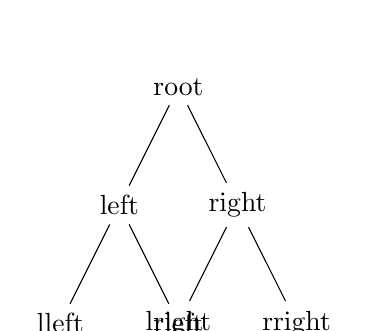
\begin{tikzpicture}
	\node {root}
	child {node {left}
			child {node {lleft}}
			child {node {rleft}}
		}
	child {node {right}
			child {node {lright}}
			child {node {rright}}
		};

\end{tikzpicture}

\newpar
Then upon evaluation, they will produce not the same values. This causes an issues
thus we must define a set of precedence with out operators.

\newpar
To maintain semantics of desired functionality, we define the following:

\begin{definition}{Precedence}{def_prec}\label{def_prec}
	\bemph{Precedence} determines which operator is evaluated first in an expression containing
	a mixture of different operators.
	Operators with higher precedence are evaluated before operators with lower precedence.
	Operators with higher precedence are said to \bemph{bind tigher}.
\end{definition}

\begin{definition}{Associativity}{def_accos}\label{def_assoc}
	\bemph{Associativity} determines which operator is evaluated first in an expression in a series of the
	\textit{same} opeartor.
	\begin{itemize}
		\item When an operator is \bemph{left-associative}, operators on the left are evaluated first before those on the right
		\item When an operator is \bemph{right-associative}, operators on the right are evaluated first before those on the right
		\item When an operator is \bemph{non-associative} this means that it's an error to use that operator more than once in a sequence.
		\item \(\exists\) languages s.t. \(\exists\) certain operators have no precedence.
	\end{itemize}
\end{definition}

\newpar
E.g. For left-associative, \(5 - 3 - 1 \equiv (5 - 3) - 1\)

\newpar
E.g. For right-associative, \(a = b = b \equiv a = (b = c)\).

\newpar
When writing source code, the writer would not need to explicity state the groupings
as the syntax tree should handle that itself to maintain semantic integrity.

\newpar
For lox, we will use the following precedence form lowest to highest as in C:
\begin{tabbing}
	\textbf{Name}  \hspace{8em} \= \textbf{Operators} \hspace{8em} \=  \textbf{Assoicates} \\
	\text{Equality}\>   == \ != \> \text{Left}\\
	\text{Comparison}\>   > \ >= \ < \ <= \> \text{Left}\\
	\text{Term}\>   - \ +  \> \text{Left}\\
	\text{Factor}\>   / \ * \> \text{Left}\\
	\text{Unary}\>   ! \ - \> \text{Right}
\end{tabbing}

\newpar
The current construction allows for the grammar to accept expressions regardless
of the defined precedence, to fix this we define in the grammar a separate rule
for each precedence level.

\newpar
Hence, we have the following grammar rules that forces the grammar to adhere to our semantics:
Primary rule holds all literals and parenthesized expressions which are at the top of precedence.
For adherance, we enforce that each production rule can only match expressions at its precedence level or higher.

\begin{tabbing}
	\texttt{expression}  \quad \= \texttt{→} \= \texttt{equality }  \\
	\texttt{equality} {→} \> \texttt{comparison ( ("==" | "!=" )  comparison )* ;} \\
	\texttt{comparison} \> \texttt{→} \> \texttt{term ( (">" | ">=" | "<" | "<=") term )* ;} \\
	\texttt{term} \> \texttt{→} \> \texttt{factor ( ("-" | "+") factor )* ;} \\
	\texttt{factor} \> \texttt{→} \> \texttt{unary ( ("/" | "*") unary )* ;} \\
	\texttt{unary} \> \texttt{→} \> \texttt{("!" | "-") unary }  \\
	\>  \texttt{| primary} \> \\
	\texttt{primary} \> \texttt{→} \>\texttt{NUMBER | STRING | "true" | "false" | "nil"} \\
	\>   \texttt{| "(" expression ")" ;}  \>
\end{tabbing}

\subsection{Recurive Descent Parsing}

\begin{definition}{Rersursive Descent Parsing}{def:rdp}\label{rdp}
	\bemph{Recurive  Descent Parsing} is a \textbf{top-down parser}.
	It starts from the outermost or top grammar rule, (expreession) and works its way down
	nested subexpressions and bottoms out at the leaves of the syntax tree.
\end{definition}

\newpar
In essence, rdp is a literaly translation of the grammar into imperative code.
Each rule is a function associated with its implementation determined by the precedence.
It is called "recursive" since grammar rules can refer to itself leading to recursive calls.









\end{document}
